\input templates/header
\title[ASD - Ricerca locale]{\textbf{Algoritmi e Strutture Dati}\\[24pt]Ricerca locale}

\usepackage{xcolor}
\usepackage{colortbl}
\usepackage{epigraph}
\usepackage{tikz}
\usetikzlibrary{trees}
\usetikzlibrary{matrix}
\usetikzlibrary{graphs}
\usetikzlibrary{shapes}
\usetikzlibrary{positioning}
\usepackage{xmpmulti}
\usepackage{listings}

\lstset{
  basicstyle=\ttfamily,
  columns=fullflexible,
  keywordstyle=\color{red}\bfseries,
  commentstyle=\color{blue},
  showstringspaces=false,
}

\tikzset{
    Node/.style = {circle, draw=black, align=center, fill=yellow!40, thick}
}    
\tikzset{
    Edge/.style = {draw=black,thick,-latex}
}    

\newcommand*\circled[1]{\tikz[baseline=(char.base)]{
            \node[circle,ball color=blue, shade, 
 color=white,inner sep=1.2pt] (char) {\tiny #1};}}

\newcommand{\R}[1]{\textcolor{red}{#1}}
\newcommand{\B}[1]{\textcolor{blue}{#1}}
\newcommand{\G}[1]{\textcolor{violet}{#1}}

\graphicspath{{figs/15/}}

\begin{document}


%-------------------------------------------------------------------------
\FrameTitle{}

%-------------------------------------------------------------------------
\FrameContent



%%%%%%%%%%%%%%%%%%%%%%%%%%%%%%%%%%%%%%%%%%%%%%%%%%%%%%%%%%%%%%%%%%%%%%%%%%
\section{Introduzione}

%-------------------------------------------------------------------------
\begin{frame}{Ricerca locale}

Se si conosce una soluzione ammissibile (non necessariamente ottima) ad un
problema di ottimizzazione, si può cercare di trovare una soluzione migliore
nelle "vicinanze" di quella precedente. Si continua in questo modo fino a
quando non si è più in grado di migliorare


\begin{Procedure}
\caption[A]{\ricercalocale()}
$\Sol = \textrm{una soluzione ammissibile del problema}$\;
\While{$\exists S \in I(\Sol)$ migliore di \Sol}
{
  $\Sol = S$\;
}
\Return \Sol\;
\end{Procedure}


\end{frame}

\begin{frame}{Ricerca locale}

\vspace{-9pt}
\begin{center}
\IG{0.85}{search.pdf}
\end{center}

\end{frame}


%%%%%%%%%%%%%%%%%%%%%%%%%%%%%%%%%%%%%%%%%%%%%%%%%%%%%%%%%%%%%%%%%%%%%%%%%%
\section{Flusso massimo}

\subsection{Rete di flusso}

%-------------------------------------------------------------------------
\begin{frame}{Rete di flusso}

\vspace{-9pt}
\begin{myboxtitle}[Definizione]
Una \alert{rete di flusso $G=(V,E,s,t,c)$} è data da:
\BI
\item un grafo orientato $G=(V,E)$
\item un nodo $s \in V$ detto \alert{sorgente}
\item un nodo $t \in V$ detto \alert{pozzo}
\item una funzione di \alert{capacità} $c: V \times V \rightarrow \mathbb{R}^{\geq 0}$,\\
tale per cui $(u,v) \not \in E \Rightarrow c(u,v)=0$.
\EI
\end{myboxtitle}

\begin{myboxtitle}[Assunzioni]
\BIL
\item Per ogni nodo $v \in V$, esiste un cammino $s \leadsto v \leadsto t$ 
da $s$ a $t$ che passa per $v$.
\item Possiamo ignorare i nodi che non godono di questa proprietà
\EIL
\end{myboxtitle}

\end{frame}

%%---------------------------------------------------------------------------
\begin{frame}{Rete di flusso}

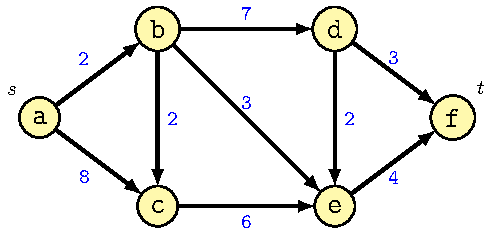
\includegraphics[width=1.0\textwidth]{template.pdf}

\end{frame}

\subsection{Flusso}

%%---------------------------------------------------------------------------
\begin{frame}{Flusso}

\vspace{-9pt}
\begin{myboxtitle}[Flusso]
Un \alert{flusso} in $G$ è una funzione \alert{$f: V \times V \rightarrow \mathbb{R}$} 
che soddisfa le seguenti proprietà:
\BIL
\item \alert{Vincolo sulla capacità}: $\forall u,v \in V$, $f(u,v) \leq c(u,v)$

\item \alert{Antisimmetria}: $\forall u,v \in V$, $f(u,v) = -f(v,u)$

\item \alert{Conservazione del flusso}: $\forall u \in V-\{s,t\}$, 
$\sum_{v \in V} f(u,v) = 0$
\EIL
\end{myboxtitle}

\end{frame}

%%---------------------------------------------------------------------------
\begin{frame}{Flusso}

\vspace{-9pt}
\begin{myboxtitle}[Vincolo sulla capacità]
Il flusso non deve eccedere la capacità sull'arco
\[
\alert{\forall u,v \in V: f(u,v) \leq c(u,v)}
\]
\end{myboxtitle}

\smallskip
\begin{center}
\IG{0.3}{prop1.pdf}
\end{center}

\end{frame}


%%---------------------------------------------------------------------------
\begin{frame}{Flusso}

\vspace{-9pt}
\begin{myboxtitle}[Antisimmetria]
\[
\alert{\forall u,v \in V: f(u,v) = -f(v,u)}
\]
Il flusso viene definito in questo modo per semplificare la proprietà successiva e altre regole.
\end{myboxtitle}

\smallskip
\begin{center}
\IG{0.3}{prop2.pdf}
\end{center}

\end{frame}

%%---------------------------------------------------------------------------
\begin{frame}{Flusso}

\vspace{-9pt}
\begin{myboxtitle}[Conservazione del flusso]
Per ogni nodo, la somma dei flussi entranti deve essere uguale alla somma dei flussi uscenti.
\[
\alert{\forall u \in V-\{s,t\}: \sum_{v \in V} f(u,v) = 0}
\]
\end{myboxtitle}

\smallskip
\begin{center}
\IG{0.4}{prop3.pdf}
\end{center}

\end{frame}

%%---------------------------------------------------------------------------
\begin{frame}{Definizioni}

\vspace{-9pt}
\begin{myboxtitle}[Valore del flusso]
Il \alert{valore di un flusso} $f$ è definito come:
\[
  |f| = \sum_{(s, v) \in E} f(s,v)
\]
ovvero come la quantità di flusso uscente da $s$.
\end{myboxtitle}

\begin{columns}[T]
\column{0.3\textwidth}
\[|f| = 3\]
\column{0.75\textwidth}
\vspace{-12pt}
\IG{0.7}{valoreflusso.pdf}
\end{columns}

\end{frame}

\subsection{Problema}

%%---------------------------------------------------------------------------
\begin{frame}{Problema}

\vspace{-9pt}
\begin{myboxtitle}[Flusso massimo]
Data una rete $G=(V,E,s,t,c)$, trovare un flusso che abbia valore massimo fra 
tutti i flussi associabili alla rete.
\[
  |f^*| = \max \{ |f| \}
\]
\end{myboxtitle}

\begin{columns}[T]
\column{0.3\textwidth}
\[|f^*| = 4\]
\column{0.75\textwidth}
\vspace{-12pt}
\IG{0.7}{flussomassimo.pdf}
\end{columns}

\end{frame}

\subsection{Metodo delle reti residue}


%%---------------------------------------------------------------------------
\begin{frame}{Metodo delle reti residue}

\vspace{-9pt}
\begin{myboxtitle}[Algoritmo, informale]
\BIL
\item Si memorizza un flusso "corrente" $f$, inizialmente nullo
\item Si ripetono le operazioni seguenti:
  \BIL
  \item Si "sottrae" il flusso attuale dalla rete iniziale, ottenendo una
    rete residua
  \item Si cerca un flusso $g$ all'interno della rete residua
  \item Si somma $g$ ad $f$
  \EIL
  fino a quando non è più possibile trovare un flusso positivo $g$
\EIL
\end{myboxtitle}

\begin{myboxtitle}[Output]
Se svolta correttamente, è possibile dimostrare che questo approccio restituisce
un flusso massimo
\end{myboxtitle}

\end{frame}



%%---------------------------------------------------------------------------
\begin{frame}{Definizioni}

\vspace{-9pt}
\begin{myboxtitle}[Flusso nullo]
Definiamo \alert{flusso nullo} la funzione 
$f_0: V \times V \rightarrow \mathbf{R}^{\geq 0}$ tale che
$f(u,v) = 0$ per ogni $u,v \in V$.
\end{myboxtitle}

\bigskip
\begin{columns}[T]
\column{0.3\textwidth}
\[|f| = 0\]
\column{0.75\textwidth}
\vspace{-12pt}
\IG{0.7}{flussonullo.pdf}
\end{columns}

\end{frame}


%-------------------------------------------------------------------------
\begin{frame}{Definizioni}

\vspace{-9pt}
\begin{myboxtitle}[Somma di flussi]
Per ogni coppia di flussi $f_1$ e $f_2$ in $G$, definiamo il \alert{flusso somma}
$g = f_1+f_2$ come un flusso tale per cui $g(u,v) = f_1(u,v) + f_2(u,v)$.
\end{myboxtitle}

\IG{0.9}{sum.pdf}

\end{frame}

%%---------------------------------------------------------------------------
\begin{frame}{Definizioni}

\vspace{-9pt}
\begin{myboxtitle}[Capacità residua]
Definiamo \alert{capacità residua} di un flusso $f$ in una rete $G=(V,E,s,t,c)$ 
una funzione $c_f: V \times V \rightarrow \mathbf{R}^{\geq 0}$
tale che $c_f(u,v) = c(u,v) - f(u,v)$.
\end{myboxtitle}

\smallskip
\begin{center}
\IG{0.4}{prop4.pdf}
\end{center}

\BI
\item Flusso in \R{rosso}
\item Capacità residua in \G{viola}
\item Capacità iniziale in \B{blu}
\EI
\end{frame}

%%---------------------------------------------------------------------------
\begin{frame}{Definizioni}

\vspace{-9pt}
\begin{myboxtitle}[Capacità residua]
Definiamo \alert{capacità residua} di un flusso $f$ in una rete $G=(V,E,s,t,c)$ 
una funzione $c_f: V \times V \rightarrow \mathbf{R}^{\geq 0}$
tale che $c_f(u,v) = c(u,v) - f(u,v)$.
\end{myboxtitle}

\smallskip
\begin{center}
\IG{0.4}{prop5.pdf}
\end{center}

Per la definizione di capacità residua, si creano degli archi all'indietro:
\begin{align*}
  c_f(b,a) &= c(b,a) - f(b,a) \\
           &= 0 - (-5)  = 5 \\
\end{align*}

\end{frame}

%%---------------------------------------------------------------------------
\begin{frame}{Definizioni}

\vspace{-9pt}
\begin{myboxtitle}[Reti residue]
Data una rete di flusso $G=(V,E,s,t,c)$ e un flusso $f$ su $G$, 
possiamo costruire una \alert{rete residua} $G_f=(V,E_f,s,t,c_f)$, tale
per cui $(u,v) \in E_f$ se e solo se $c_f(u,v) > 0$. 
\end{myboxtitle}

\smallskip
\begin{center}
\IG{0.7}{reteresidua.pdf}
\end{center}

\end{frame}

\subsection{Algoritmo}

%%---------------------------------------------------------------------------
\begin{frame}{Algoritmo, schema generale}

\begin{Procedure}
\caption[A]{$\INTARRAY[\,]$ \Flusso(\Graph $G$, \Node $s$, \Node $t$, $\INTARRAY[\,]\ c$)}
$f = f_0$\REMR{Inizializza un flusso nullo}
$r = c$\REMR{Capacità iniziale}
\Repeat{$g = f_0$}{
  $g = \textrm{trova un flusso in $r$ tale che $|g| > 0$, altrimenti $f_0$}$\;
  $f = f + g$\;
  $r = \textrm{Rete di flusso residua del flusso $f$ in $G$}$\;
}
\Return $f$
\end{Procedure}

\end{frame}

%%---------------------------------------------------------------------------
\begin{frame}{Dimostrazione correttezza}

\vspace{-9pt}
\begin{myboxtitle}[Lemma]
Se $f$ è un flusso in $G$ e $g$ è un flusso in $G_f$, allora
$f+g$ è un flusso in $G$.
\end{myboxtitle}

\BB{Vincolo sulla capacità}
\begin{align*}
g(u,v) &\leq c_f(u,v) & \textrm{\small $g$ è un flusso in $G_f$} \\
\alert{f(u,v)} + g(u,v) &\leq  c_f(u,v) + \alert{f(u,v)} & \textrm{\small Aggiungo termine uguale}\\
(f+g)(u,v) &\leq c(u,v)-f(u,v) + f(u,v) & \textrm{\small Sostituzione}\\
(f+g)(u,v) &\leq c(u,v) & \textrm{\small Semplificazione}
\end{align*}

\end{frame}

%%---------------------------------------------------------------------------
\begin{frame}{Dimostrazione correttezza}

\vspace{-9pt}
\begin{myboxtitle}[Lemma]
Se $f$ è un flusso in $G$ e $g$ è un flusso in $G_f$, allora
$f+g$ è un flusso in $G$.
\end{myboxtitle}

\BB{Antisimmetria}
\begin{align*}
f(u,v)+g(u,v) &= -f(v,u)-g(v,u) & \textrm{\small Antisimmetria $f$, $g$} \\
f(u,v)+g(u,v) &= -(f(v,u) + g(v,u)) & \textrm{\small Raccolta segno $-$} \\
(f+g)(u,v) &= -(f+g)(v,u) & \textrm{\small Sostituzione} 
\end{align*}

\end{frame}

%%---------------------------------------------------------------------------
\begin{frame}{Dimostrazione correttezza}

\vspace{-9pt}
\begin{myboxtitle}[Lemma]
Se $f$ è un flusso in $G$ e $g$ è un flusso in $G_f$, allora
$f+g$ è un flusso in $G$.
\end{myboxtitle}

\BB{Conservazione}

\begin{align*}
  \sum_{v \in V} (f+g)(u,v) &= \sum_{v \in V} (f(u,v) + g(u,v)) \\
  &= \sum_{v \in V} f(u,v) + \sum_{v \in V} g(u,v) \\
   &= 0
\end{align*}

\end{frame}

%%---------------------------------------------------------------------------
\begin{frame}{Metodo dei cammini aumentanti}

\vspace{-9pt}
\BB{Domanda}
Il punto principale del metodo precedente è il seguente: come trovare un 
flusso aggiuntivo? 

\begin{center}
\IG{0.8}{template.pdf}
\end{center}

\end{frame}

%%---------------------------------------------------------------------------
\begin{frame}{Ford-Fulkerson, 1956}

\vspace{-9pt}
\begin{overprint}
\onslide<1|handout:1>
\BIL
\item Si trova un cammino $C=v_0,v_1,\ldots,v_n$, con $s=v_0$ e $t=v_n$ 
  nella rete residua $G_f$; 
\item Si identifica la \alert{capacità del cammino}, corrispondente
  alla minore capacità degli archi incontrati (collo di bottiglia):
  \[
    c_f(C) = \min_{i=2 \ldots n} c_f(v_{i-1},v_i)
  \]
\EIL
\onslide<2|handout:2>
\BIL
\item si crea un flusso addizionale $g$ tale che 
  \BI
  \item $g(v_{i-1}, v_i) = c_f(C)$;
  \item $g(v_i,v_{i-1}) = -c_f(C)$ (per antisimmetria)
  \item $g(x,y)=0$ per tutte le altre coppie $(x,y)$
  \EI
\EIL
\end{overprint}

\medskip
\begin{overprint}
\onslide<1|handout:1>
\begin{center}
\IG{0.7}{cammino-aumentante.pdf}
\end{center}
\onslide<2|handout:2>
\begin{center}
\IG{0.7}{flusso-aumentante.pdf}
\end{center}
\end{overprint}



\end{frame}

%%---------------------------------------------------------------------------
\begin{frame}{Ford-Fulkerson, 1956}

\vspace{-9pt}
\begin{Procedure}
\caption[A]{$\INTARRAY[\,]$ \Flusso(\Graph $G$, \Node $s$, \Node $t$, $\INTARRAY[\,]\ c$)}
$\INTARRAY[\,]\ f = \NEW\ \INTARRAY[\,]$\REMR{Flusso parziale}
$\INTARRAY[\,]\ g = \NEW\ \INTARRAY[\,]$\REMR{Flusso da cammino aumentante}
$\INTARRAY[\,]\ r = \NEW\ \INTARRAY[\,]$\REMR{Rete residua}
\BlankLine
\ForEach{$u,v \in G.\VV()$}{
  $f[u][v] = 0$\REMR{Inizializza un flusso nullo}
  $r[u][v] = c[u][v]$\REMR{Copia c in r}
}
\Repeat{$g=f_0$}{
  $g = \textrm{flusso associato ad un cammino aumentante in $r$, oppure $f_0$}$\;
  \ForEach{$u,v \in G.\VV()$}{
    $f[u][v] = f[u][v] + g[u][v]$\REMR{$f = f + g$}
    $r[u][v] = c[u][v] - f[u][v]$\REMR{Calcola $c_f$}
  }  
}
\Return $f$
\end{Procedure}

\end{frame}

%%---------------------------------------------------------------------------
\begin{frame}{Esecuzione}

\begin{columns}[T]
\column{0.75\textwidth}
\begin{overprint}
\includegraphics<1|handout:1>[width=\textwidth,page=1]{esempio.pdf}
\includegraphics<2|handout:2>[width=\textwidth,page=2]{esempio.pdf}
\includegraphics<3|handout:0>[width=\textwidth,page=3]{esempio.pdf}
\includegraphics<4|handout:0>[width=\textwidth,page=4]{esempio.pdf}
\includegraphics<5|handout:0>[width=\textwidth,page=5]{esempio.pdf}
\includegraphics<0|handout:3>[width=\textwidth,page=17]{esempio.pdf}
\includegraphics<6|handout:4>[width=\textwidth,page=6]{esempio.pdf}
\includegraphics<7|handout:0>[width=\textwidth,page=7]{esempio.pdf}
\includegraphics<8|handout:0>[width=\textwidth,page=8]{esempio.pdf}
\includegraphics<9|handout:0>[width=\textwidth,page=9]{esempio.pdf}
\includegraphics<0|handout:5>[width=\textwidth,page=18]{esempio.pdf}
\includegraphics<10|handout:6>[width=\textwidth,page=10]{esempio.pdf}
\includegraphics<11|handout:0>[width=\textwidth,page=11]{esempio.pdf}
\includegraphics<12|handout:0>[width=\textwidth,page=12]{esempio.pdf}
\includegraphics<13|handout:0>[width=\textwidth,page=13]{esempio.pdf}
\includegraphics<14|handout:0>[width=\textwidth,page=14]{esempio.pdf}
\includegraphics<15|handout:0>[width=\textwidth,page=15]{esempio.pdf}
\includegraphics<0|handout:7>[width=\textwidth,page=16]{esempio.pdf}
\end{overprint}
\column{0.20\textwidth}
\begin{overprint}
\onslide<3|handout:0>
\B{$f(\mathtt{a},\mathtt{b}) = 2$}\\
\onslide<4|handout:0>
$f(\mathtt{a},\mathtt{b}) = 2$\\
\B{$f(\mathtt{b},\mathtt{e}) = 2$}\\
\onslide<5|handout:0>
$f(\mathtt{a},\mathtt{b}) = 2$\\
$f(\mathtt{b},\mathtt{e}) = 2$\\
\B{$f(\mathtt{e},\mathtt{f}) = 2$}\\
\onslide<6|handout:3-4>
$f(\mathtt{a},\mathtt{b}) = 2$\\
$f(\mathtt{b},\mathtt{e}) = 2$\\
$f(\mathtt{e},\mathtt{f}) = 2$\\
\onslide<7|handout:0>
$f(\mathtt{a},\mathtt{b}) = 2$\\
$f(\mathtt{b},\mathtt{e}) = 2$\\
$f(\mathtt{e},\mathtt{f}) = 2$\\
\B{$f(\mathtt{a},\mathtt{c}) = 2$}\\
\onslide<8|handout:0>
$f(\mathtt{a},\mathtt{b}) = 2$\\
$f(\mathtt{b},\mathtt{e}) = 2$\\
$f(\mathtt{e},\mathtt{f}) = 2$\\
$f(\mathtt{a},\mathtt{c}) = 2$\\
\B{$f(\mathtt{c},\mathtt{e}) = 2$}\\
\onslide<9|handout:0>
$f(\mathtt{a},\mathtt{b}) = 2$\\
$f(\mathtt{b},\mathtt{e}) = 2$\\
\B{$f(\mathtt{e},\mathtt{f}) = \xout{2} \ 4$}\\
$f(\mathtt{a},\mathtt{c}) = 2$\\
$f(\mathtt{c},\mathtt{e}) = 2$\\
\onslide<10|handout:5-6>
$f(\mathtt{a},\mathtt{b}) = 2$\\
$f(\mathtt{b},\mathtt{e}) = 2$\\
$f(\mathtt{e},\mathtt{f}) = \xout{2} \ 4$\\
$f(\mathtt{a},\mathtt{c}) = 2$\\
$f(\mathtt{c},\mathtt{e}) = 2$\\
\onslide<11|handout:0>
$f(\mathtt{a},\mathtt{b}) = 2$\\
$f(\mathtt{b},\mathtt{e}) = 2$\\
$f(\mathtt{e},\mathtt{f}) = \xout{2} \ 4$\\
\B{$f(\mathtt{a},\mathtt{c}) = \xout{2} \ 4$}\\
$f(\mathtt{c},\mathtt{e}) = 2$\\
\onslide<12|handout:0>
$f(\mathtt{a},\mathtt{b}) = 2$\\
$f(\mathtt{b},\mathtt{e}) = 2$\\
$f(\mathtt{e},\mathtt{f}) = \xout{2} \ 4$\\
$f(\mathtt{a},\mathtt{c}) = \xout{2} \ 4$\\
\B{$f(\mathtt{c},\mathtt{e}) = \xout{2} \ 4$}\\
\onslide<13|handout:0>
$f(\mathtt{a},\mathtt{b}) = 2$\\
\B{$f(\mathtt{b},\mathtt{e}) = \xout{2} \ 0$}\\
$f(\mathtt{e},\mathtt{f}) = \xout{2} \ 4$\\
$f(\mathtt{a},\mathtt{c}) = \xout{2} \ 4$\\
$f(\mathtt{c},\mathtt{e}) = \xout{2} \ 4$\\
\onslide<14|handout:0>
$f(\mathtt{a},\mathtt{b}) = 2$\\
$f(\mathtt{b},\mathtt{e}) = \xout{2} \ 0$\\
$f(\mathtt{e},\mathtt{f}) = \xout{2} \ 4$\\
$f(\mathtt{a},\mathtt{c}) = \xout{2} \ 4$\\
$f(\mathtt{c},\mathtt{e}) = \xout{2} \ 4$\\
\B{$f(\mathtt{b},\mathtt{d}) = 2$}\\
\onslide<15|handout:0>
$f(\mathtt{a},\mathtt{b}) = 2$\\
$f(\mathtt{b},\mathtt{e}) = \xout{2} \ 0$\\
$f(\mathtt{e},\mathtt{f}) = \xout{2} \ 4$\\
$f(\mathtt{a},\mathtt{c}) = \xout{2} \ 4$\\
$f(\mathtt{c},\mathtt{e}) = \xout{2} \ 4$\\
$f(\mathtt{b},\mathtt{d}) = 2$\\
\B{$f(\mathtt{d},\mathtt{f}) = 2$}\\
\onslide<0|handout:7>
$f(\mathtt{a},\mathtt{b}) = 2$\\
$f(\mathtt{b},\mathtt{e}) = \xout{2} \ 0$\\
$f(\mathtt{e},\mathtt{f}) = \xout{2} \ 4$\\
$f(\mathtt{a},\mathtt{c}) = \xout{2} \ 4$\\
$f(\mathtt{c},\mathtt{e}) = \xout{2} \ 4$\\
$f(\mathtt{b},\mathtt{d}) = 2$\\
$f(\mathtt{d},\mathtt{f}) = 2$\\
\end{overprint}

\end{columns}

\end{frame}


%%---------------------------------------------------------------------------
\begin{frame}{Ricerca del cammino}

Ford e Fulkerson suggerirono una semplice visita del grafo, in profondità 
oppure in ampiezza.

\bigskip
Edmonds e Karp suggerirono di utilizzare una visita in ampiezza.

\bigskip
Costo della visita: $O(V+E)$


\end{frame}

%%---------------------------------------------------------------------------
\begin{frame}[fragile]{Ricerca del cammino}

\vspace{-12pt}
\small
\begin{lstlisting}[language=java]    
/**
 * Compute the max-flow using the Ford-Fulkerson algorithm
 * @param C the capacity matrix
 * @param s the source node
 * @param t the sink node
 * @return the flow matrix 
 */
private static int[][] flow(int[][] C, int s, int t) {
  // Create an empty flow
  int[][] F = new int[C.length][C.length];
  // Visited array to perform DFS, initially empty
  boolean[] visited = new boolean[C.length];
  // Repeat until there is no path    
  while (dfs(C, F, s, t, visited, Integer.MAX_VALUE) > 0) {
    Arrays.fill(visited, false);
  }
  return F;
}
\end{lstlisting}

\end{frame}

%%---------------------------------------------------------------------------
\begin{frame}[fragile,shrink=5]{Ricerca del cammino}

\vspace{-15pt}
\footnotesize
\begin{lstlisting}[language=java]    
/**
 * Performs a DFS starting from node i and trying to reach node t. 
 * @param C the capacity matrix; if capacity[x][y]>0, there is a edge from x to y
 * @param F the flow matrix to be computed
 * @param i the current node, 
 * @param t the sink node
 * @param visited the boolean set containing the nodes that have been visited
 * @param min the smallest capacity found during the visit.
 * @returns the value of the additional flow found during the DFS
 */
private static int dfs(int[][] C, int[][] F, int i, int t, boolean[] visited, int min) {
  if (i==t) return min;             // If sink has been reached, terminate
  visited[i] = true;
  for (int j=0; j < C.length; j++) {
    if (C[i][j] > 0 && !visited[j]) {    // Non-visited neighbor
      int val = dfs(C, F, j, t, visited, Math.min(min, C[i][j]));
      if (val > 0) {
        C[i][j] = C[i][j]-val; C[j][i] = C[j][i]+val;
        F[i][j] = F[i][j]+val; F[j][i] = F[j][i]-val;
        return val;
      }
    }
  }  
  return 0;                 // The sink has not been found
}
\end{lstlisting}

\end{frame}





\subsection{Complessità}


%%---------------------------------------------------------------------------
\begin{frame}{Complessità}

\vspace{-3pt}
\begin{myboxtitle}[Complessità, limite superiore -- Versione Ford-Fulkerson]
Se le capacità sono intere, l'algoritmo di Ford-Fulkerson
ha complessità \alert{$O((V+E)|f^*|)$} (liste) o \alert{$O(V^2|f^*|)$} (matrice).
\end{myboxtitle}

\BIL
\item L'algoritmo parte dal flusso nullo e termina quando il valore totale
del flusso raggiunge $|f^*|$
\item Ogni incremento del flusso aumenta il flusso di almeno un'unità
\item Ogni ricerca di un cammino richiede una visita del grafo, con
costo $O(V+E)$ o $O(V^2)$; 
\item La somma dei flussi e il calcolo della rete residua può essere 
effettuato in tempo $O(V+E)$ o $O(V^2)$.
\EIL

\end{frame}

%%---------------------------------------------------------------------------
\begin{frame}{Complessità}

\vspace{-3pt}
\begin{myboxtitle}[Complessità, limite superiore -- Edmonds e Karp]
Se le capacità della rete sono intere, l'algoritmo di Edmonds e Karp
ha complessità \alert{$O(VE^2)$} nel caso pessimo.
\end{myboxtitle}

\BB{Come si conciliano i due limiti superiori?}

\BIL
\item $O(VE^2)$ vs $O((V+E)|f^*|)$
\item Sono entrambi limiti superiori
\item Sono entrambi validi
\item Si deve quindi prendere il più basso fra i due
\EIL

\end{frame}

%-------------------------------------------------------------------------
\begin{frame}{Dimostrazione complessità}

\vspace{-9pt}
\begin{myboxtitle}[Teorema]
La complessità dell'algoritmo di Edmonds-Karp è $O(VE^2)$.
\end{myboxtitle}
\BIL
\item Vengono eseguiti $O(VE)$ aumenti di flusso, ognuno dei quali richiede
una visita in ampiezza $O(V+E)$.
\item $O(VE(V+E)) = O(VE^2)$
\EIL

% \begin{myboxtitle}[Lemma - Aumenti di flusso]
% Il numero totale di aumenti di flusso eseguiti dall'algoritmo
% di Edmonds e Karp è $O(VE)$.
% \end{myboxtitle}

\end{frame}

%-------------------------------------------------------------------------
\begin{frame}{Dimostrazione complessità}

\vspace{-9pt}
\begin{myboxtitle}[Lemma - Monotonia]
Sia $\delta_f(s,v)$ la distanza minima da $s$ a $v$ in una rete residua $G_f$.
Sia $f' = f+g$ un flusso nella rete iniziale, con $g$ flusso non nullo derivante
da un cammino aumentante. Allora $\delta_{f'}(s,v) \geq \delta_f(s,v)$.
\end{myboxtitle}  
\BI
  \item Quando viene aumentato il flusso, alcuni archi si  ``spengono'' (capacità residua 0)
  \item Questi archi erano utilizzati nei cammini minimi (BFS)
  \item I cammini minimi non posso diventare più corti
\EI

\begin{overprint}
\onslide<1|handout:1>
\begin{center}
\includegraphics[width=0.6\textwidth,page=1]{bfs.pdf}
\end{center}
\onslide<2|handout:2>
\begin{center}
\includegraphics[width=0.6\textwidth,page=2]{bfs.pdf}
\end{center}
\onslide<3|handout:3>
\begin{center}
\includegraphics[width=0.6\textwidth,page=3]{bfs.pdf}
\end{center}
\end{overprint}

\end{frame}

%-------------------------------------------------------------------------
\begin{frame}{Dimostrazione complessità}

\vspace{-9pt}
\begin{myboxtitle}[Lemma - Aumenti di flusso]
Il numero totale di aumenti di flusso eseguiti dall'algoritmo
di Edmonds e Karp è $O(VE)$.
\end{myboxtitle}

\BIL
\item Sia $G_f$ una rete residua
\item Sia $C$ un cammino aumentante di $G_f$. 
\item $(u,v)$ è un arco \alert{critico} (collo di bottiglia) in $C$ se 

\[
c_f(u,v) = \min_{(x,y \in C)} \{ c_f(x,y) \}
\]

\item In ogni cammino esiste almeno un arco critico
\item Una volta aggiunto il flusso associato a $C$, l'arco critico scompare dalla rete residua. 
\EIL

\end{frame}

%-------------------------------------------------------------------------
\begin{frame}{Dimostrazione complessità}

\BIL
\item Poiché i cammini aumentanti sono cammini minimi, abbiamo che:
\[
 \delta_f(s,v) = \delta_f(s,u)+1
\]
\item L'arco $(u,v)$ potrà ricomparire se e solo se il flusso lungo l'arco 
diminuirà, ovvero se $(v,u)$ appare in un cammino aumentante
\item  Sia $g$ il flusso quando questo accade; come sopra, abbiamo:
\[
 \delta_{g}(s,u) = \delta_{g}(s,v)+1
\]
\item Per Lemma (Monotonia), abbiamo anche che $\delta_g(s,v)
\geq \delta_{f}(s,v)$; quindi:
\begin{eqnarray*}
\delta_{g}(s,u) &=& \delta_{g}(s,v)+1 \\
  & \geq & \delta_f(s,v) + 1 \\
  & \geq & \delta_f(s,u) + 2
\end{eqnarray*}
\EIL

\end{frame}

%-------------------------------------------------------------------------
\begin{frame}{Dimostrazione complessità}

\BIL
\item Dal momento in cui un nodo è critico al momento in cui può tornare ad essere critico , il cammino minimo si è allungato almeno di due passi.
\item La lunghezza massima del cammino fino a $u$, tenuto conto che poi si deve ancora seguire l'arco $(u,v)$,
è $V-2$. 
\item Quindi un arco può diventare critico al massimo $(V-2)/2 = V/2-1$ volte. 
\item Poiché ci sono $O(E)$ archi che possono diventare critici $O(V)$ volte,
abbiamo che il numero massimo di flussi aumentanti è $O(VE)$. 
\EIL

\end{frame}


%%---------------------------------------------------------------------------
\begin{frame}{Complessità -- Altre versioni}

\small
\begin{tabular}{|P{2.6cm}|P{3.5cm}|P{4.1cm}|}
\hline
\textbf{Nome} & \textbf{Complessità} & \textbf{Note} \\\hline
Ford-Fulkerson & $O(E|f^*|)$ & Converge con valori razionali \\\hline
Edmonds-Karp & $O(VE^2)$ & Specializzazione basata su BFS \\\hline
Dinic, blocking flow & $O(V^2E)$ & In alcune reti particolari, $O((V^{2/3},E^{1/2})E)$ \\\hline
MPM & $O(V^3)$ & Solo su DAG \\\hline
Dinic & $O(VE \log V)$ & Struttura dati Dynamic trees \\\hline
Goldberg e Rao & \begingroup \footnotesize $O(\min(n^{2/3},m^{1/2})m \cdot {}$ \endgroup & $C=\max_{(u,v) \in E} c(u,v)$ \\
& \begingroup \footnotesize  ${} \cdot \log (n^2/m+2) \log C)$ \endgroup & \\\hline

Orlin + King,Rao,Tarjan & $O(VE)$ & Pubblicato nel 2013!\\\hline
\end{tabular}

\end{frame}


%%%%%%%%%%%%%%%%%%%%%%%%%%%%%%%%%%%%%%%%%%%%%%%%%%%%%%%%%%%%%%%%%%%%%%%%%%%%%
\subsection{Dimostrazione di correttezza}

%%---------------------------------------------------------------------------
\begin{frame}{Dimostrazione correttezza -- Definizioni}

\vspace{-12pt}
\begin{myboxtitle}[Taglio]
Un \alert{taglio} $(S,T)$ della rete di flusso 
$G=(V,E,s,t,c)$ è una partizione di $V$ in $S$ e $T=V-S$
tale che $s \in S$ e $t \in T$.
\end{myboxtitle}

\vspace{-12pt}
\begin{columns}[T]
\column{0.70\textwidth}
\IG{1.0}{taglio.pdf}
\column{0.28\textwidth}
\vspace{18pt}
$S = \{ \mathtt{a}, \mathtt{b}, \mathtt{c}, \mathtt{d} \}$\\
$T = \{ \mathtt{e}, \mathtt{f} \}$\\
\end{columns}


\end{frame}


%%---------------------------------------------------------------------------
\begin{frame}{Dimostrazione correttezza -- Definizioni}

\vspace{-12pt}
\begin{myboxtitle}[Capacità di un taglio]
La \alert{capacità} $C(S,T)$ attraverso il taglio $(S,T)$ è pari a:

\[
  C(S,T) = \sum_{u \in S, v \in T} c(u,v)
\]
\end{myboxtitle}

\vspace{-12pt}
\begin{columns}[T]
\column{0.70\textwidth}
\IG{1.0}{taglio2.pdf}
\column{0.28\textwidth}
\vspace{18pt}
$S = \{ \mathtt{a}, \mathtt{b}, \mathtt{c}, \mathtt{d} \}$\\
$T = \{ \mathtt{e}, \mathtt{f} \}$\\
~\\
$C(S,T) = 14$
\end{columns}

\end{frame}

%%---------------------------------------------------------------------------
\begin{frame}{Dimostrazione correttezza -- Definizioni}

\vspace{-9pt}
\begin{myboxtitle}[Flusso di un taglio]
Se $f$ è un flusso in $G$, il {\em flusso netto} $F(S,T)$ 
attraverso $(S,T)$ è:

\[
  F(S,T) = \sum_{u \in S, v \in T} f(u,v)
\]
\end{myboxtitle}

\vspace{-12pt}
\begin{columns}[T]
\column{0.70\textwidth}
\IG{1.0}{taglio3.pdf}
\column{0.28\textwidth}
\vspace{18pt}
$S = \{ \mathtt{a}, \mathtt{b}, \mathtt{c}, \mathtt{d} \}$\\
$T = \{ \mathtt{e}, \mathtt{f} \}$\\
~\\
$C(S,T) = 14$\\
~\\
$F(S,T) = 6$
\end{columns}

\end{frame}

%%---------------------------------------------------------------------------
\begin{frame}{Dimostrazione correttezza -- Lemma    }
    
\vspace{-3pt}
\begin{myboxtitle}[Lemma -- Valore del flusso di un taglio]
Dato un flusso $f$ e un taglio $(S,T$), la quantità di flusso
$F(S,T)$ che attraversa il taglio è uguale a $|f|$.
\end{myboxtitle}

\medskip
\begin{overprint}
\onslide<1|handout:1>
\IG{0.8}{taglio4.pdf}
\onslide<2|handout:2>
\begin{align*}
F(S,T) &= \sum_{u \in S, v \in T} f(u,v) \\
       &= \sum_{u \in S, v \in V} f(u,v) - \sum_{u \in S, v \in S} f(u,v)& T = V - S\\ 
       &= \sum_{u \in S, v \in V} f(u,v)& \textrm{Antisimmetria}\\
       &= [...] 
\end{align*}
\onslide<3|handout:3>
\begin{align*}
F(S,T) &= \sum_{u \in S, v \in V} f(u,v)& \\ 
       &= \sum_{u \in S-\{s\}, v \in V} f(u,v) + \sum_{v \in V} f(s,v) & s \in S\\ 
       &= \sum_{v \in V} f(s,v) & \textrm{Conservazione flusso}\\ 
       &= |f| & \textrm{Definizione valore flusso}
\end{align*}
\end{overprint}
        
\end{frame}




%%---------------------------------------------------------------------------
\begin{frame}{Dimostrazione -- Flusso massimo, taglio minimo}

\vspace{-3pt}
\begin{myboxtitle}[Lemma -- Capacità taglio]
Il \alert{flusso massimo} è limitato superiormente dalla capacità del \alert{taglio minimo}, ovvero il taglio la cui capacità è minore fra tutti i tagli.
\end{myboxtitle}

\begin{overprint}
\onslide<1|handout:1>
\IG{0.8}{minmax.pdf}
\onslide<2|handout:2>

\medskip
\BIL
\item Nessun flusso attraverso un taglio supera la capacità del taglio
\smallskip
\[
  F(S,T) \leq C(S,T) \qquad \forall S \subseteq V, T = V-S
\]
Dimostrazione:
\smallskip
\[
  F(S,T) = \sum_{u \in S, v \in T} f(u,v) \leq \sum_{u \in S, v \in T} c(u,v) = C(S,T)
\]
\item Il flusso che attraversa un taglio è uguale al valore del flusso
\smallskip
\[
  |f| = F(S,T) \qquad \forall S \subseteq V, T = V-S
\]
\EIL
\onslide<3|handout:3>

\medskip
\BIL
\item Quindi, il valore del flusso è limitato superiormente dalla capacità
di tutti i possibili tagli. 
\smallskip
\[
|f| \leq C(S,T) \qquad \forall S \subseteq V, T = V-S
\]
\EIL
\end{overprint}

\end{frame}

%%---------------------------------------------------------------------------
\begin{frame}{Teorema del taglio minimo / flusso massimo}

\vspace{-9pt}
\begin{myboxtitle}[Teorema]
Le seguenti tre affermazioni sono equivalenti:
\begin{enumerate}
\item $f$ è un \alert{flusso massimo}
\item non esiste nessun cammino aumentante per $G$
\item esiste un \alert{taglio minimo} $(S,T)$ tale che $C(S,T) = |f|$
\end{enumerate}
\end{myboxtitle}

\bigskip
Dimostreremo circolarmente:
\BIL
\item $(1) \Rightarrow (2)$
\item $(2) \Rightarrow (3)$
\item $(3) \Rightarrow (1)$
\EIL

\end{frame}

%-------------------------------------------------------------------------
\begin{frame}{Dimostrazione correttezza -- $(1) \Rightarrow (2)$}

\BB{$f$ è un flusso massimo $\Rightarrow$ non esiste nessun cammino aumentante per $G$}

\BIL
\item Se esistesse un cammino aumentante, il flusso potrebbe essere aumentato e quindi non sarebbe massimo (assurdo).
\EIL

\end{frame}

%-------------------------------------------------------------------------
\begin{frame}{Dimostrazione correttezza -- $(2) \Rightarrow (3)$}

\vspace{-9pt}
\BB{Non esiste nessun cammino aumentante per $G$ $\Rightarrow$\\
esiste un taglio minimo $(S,T)$ tale che $C(S,T) = |f|$}


\begin{center}
\IG{0.6}{dim1.pdf}
\end{center}

\small
\BI
\item Poiché non esiste nessun cammino aumentante per $f$, non esiste nessun cammino
da $s$ a $t$ nella rete residua $G_f$
\item Sia $S$ l'insieme dei vertici raggiungibili da $s$; $T=V-S$
\item Ovviamente $s \in S$ e $t \in T$, quindi $(S,T)$ è un taglio
\EI

\end{frame}


%-------------------------------------------------------------------------
\begin{frame}{Dimostrazione correttezza -- $(2) \Rightarrow (3)$}

\vspace{-9pt}
\BB{Non esiste nessun cammino aumentante per $G$ $\Rightarrow$\\
esiste un taglio minimo $(S,T)$ tale che $C(S,T) = |f|$}

\begin{center}
\IG{0.6}{dim2.pdf}
\end{center}

\small
\BI
\item Poiché $t$ non è raggiungibile da $s$ in $G_f$, tutti gli
archi $(u,v)$ con $u \in S$ e $v \in T$ sono saturati;  ovvero, $f(u,v) = c(u,v)$. 
\EI

\end{frame}

%-------------------------------------------------------------------------
\begin{frame}{Dimostrazione correttezza -- $(2) \Rightarrow (3)$}

\vspace{-9pt}
\BB{Non esiste nessun cammino aumentante per $G$ $\Rightarrow$\\
esiste un taglio minimo $(S,T)$ tale che $C(S,T) = |f|$}

\BIL
\item Per il Lemma -- Valore del flusso di un taglio,

\[ 
  |f| = \sum_{u \in S, v \in T} f(u,v)
\]
\item Ne segue che:

\[ 
  |f| = \sum_{u \in S, v \in T} f(u,v) = \sum_{u \in S, v \in t} c(u,v) = C(S,T)
\]

\item $(S,T)$ è minimo perchè $|f|=C(S,T)$ e per ogni taglio $(S', T')$, abbiamo che $|f| >= C(S', T')$

\EIL

\end{frame}

%-------------------------------------------------------------------------
\begin{frame}{Dimostrazione correttezza -- $(3) \Rightarrow (1)$}

\vspace{-9pt}
\BB{Esiste un taglio $(S,T)$ tale che $C(S,T) = |f|$ $\Rightarrow$\\
$f$ è un flusso massimo}

\bigskip
Poiché per un qualsiasi flusso $f$ e un qualsiasi taglio $(S,T)$ vale la relazione $|f| \leq C(S,T)$, 
il flusso che soddisfa $|f| = C(S,T)$ deve essere massimo.

\end{frame}

\section{Applicazioni}

%-------------------------------------------------------------------------
\begin{frame}{Applicazioni}

\begin{columns}[T]
\column{0.45\textwidth}
\BIL
\item Bipartite matching
\item Data mining
\item Project selection
\item Airline scheduling
\item Baseball elimination
\item Image segmentation
\item Network connectivity
\EIL
\column{0.45\textwidth}
\BIL
\item Network reliability
\item Distributed computing
\item Egalitarian stable matching
\item Security of statistical data
\item Network intrusion detection
\item Multi-camera scene reconstruction
\item Gene function prediction
\EIL
\end{columns}

\end{frame}

\subsection{Abbinamento grafi bipartiti}

%-------------------------------------------------------------------------
\begin{frame}{Abbinamento (matching) massimo nei grafi bipartiti}

\vspace{-9pt}
\begin{myboxtitle}[Problema - Job Assignment - Input]
\BIL
\item Un insieme $J$ contenente $n$ job
\item Un insieme $W$ contenente $m$ worker
\item Una relazione $R \subseteq J \times W$, tale per cui $(j,w) \in R$
se e solo se il job $j$ può essere useguito dal worker $w$
\EIL
\end{myboxtitle}

\begin{myboxtitle}[Problema - Job Assignment - Output]
\BIL
\item Il più grande sottoinsieme $O \subseteq R$, tale per cui:
  \BI
  \item ogni job venga assegnato al più ad un worker
  \item ad ogni worker venga assegnato al più un job
  \EI
\EIL
\end{myboxtitle}

\end{frame}
  
%-------------------------------------------------------------------------
\begin{frame}{Esempio}

\begin{overprint}
\onslide<1|handout:1>
\begin{center}
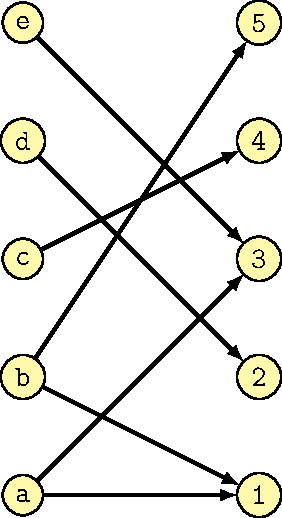
\includegraphics[height=7cm,page=1]{bipartite.pdf}
\end{center}
\onslide<2|handout:2>
\begin{center}
\includegraphics[height=7cm,page=2]{bipartite.pdf}
\end{center}
\end{overprint}
  
\end{frame}
    
\end{document}
